A common technique in physics and mathematics for solving complicated problems is to find a different way to represent the quantities involved. Familiar examples include solving a system of linear equations by arranging the coefficients in a matrix and making use of linear algebra, or determining the result of interactions in simple billiard-ball style dynamic systems using conservation of energy instead of sums of forces. The technique we discuss here is the process of representing a mathematical function (or signal, or time series) as a composition of sinusoids. This change of representation allows simplified solutions to problems ranging across countless disciplines, as well as a method for signal decomposition and analysis. There are four primary expressions of Fourier decomposition, depending on whether the input and output signals are continuous or discrete.

\subsection{Fourier Series}
The Fourier Series is the simplest form of Fourier decomposition to understand. Consider a periodic function $x(t)$. Recall that a function is periodic if there exists a number $T\in \mathbb{R}$ such that $x(t+nT) = x(t)$ for all $n \in \mathbb{Z}$. The Fourier Series associated with this function is given by
\[
x(t) = \sum_{k=0}^{\infty}(a_k \sin(k\omega_0t) + b_k \cos(k\omega_0t))
\]
The Fourier coefficients $a_k$ and $b_k$ describe how much each frequency $k\omega_0$ contributes to the function. The fundamental angular frequency $\omega_0$ is determined by the period, i.e. $\omega_0 = 2\pi/T$. It is common to express the series as a single summation over complex sinusoids instead of over sines and cosines, i.e.
\[
x(t) = \sum_{k=-\infty}^{\infty}c_k e^{ik\omega_0t}
\]
The simplification to one set of coefficients $c_k$ is offset by an extension of the summation variable $k$ to start from $-\infty$ instead of $0$. The is the well known \textbf{Fourier Series}, which, given a continuous function $x(t)$, is a discrete function of the frequency multiplier $k$. The coefficients $c_k$ are given by the inner product of $x(t)$ with a particular frequency $\exp{(-ik\omega_0t)}$, e.g.
\[
X[k] = c_k = \langle x(t),e^{ik\omega_0t}\rangle = \dfrac{1}{T}\int_{0}^{T} x(t) e^{-ik\omega_0t} dt 
\]

\subsection{Fourier Transform}
The next step is to allow the period $T$ grow to infinity. In this case, the fundamental frequency $\omega_0$ shrinks toward zero. By holding certain quantities constant in this limit, what was previously a summation becomes an integration, and we can now represent arbitrary (not necessarily periodic) functions by the Fourier integral:
\[
x(t) = \dfrac{1}{2\pi}\int_{-\infty}^{\infty}X(\omega) e^{i\omega t}d\omega
\]
The \textbf{Fourier Transform} refers to the coefficients, which have become a continuous function $X(\omega)$, determined again by the inner product:
\[
X(\omega) = \langle x(t),e^{i\omega t}\rangle = \int_{-\infty}^{\infty} x(t) e^{-i\omega t} dt 
\]
This remarkable formula now allows us to decompose any function $x(t)$ into the superposition of an infinite number of complex sinusoids. This is useful in a large number of technical fields, not least of which is mathematics: the special case of transforming the derivative of a function results in changing a differential equation into an algebraic equation. For this reason, Fourier transforms are a fundamental tool in the solutions of partial differential equations. In this case, both the input signal and the output transform are continuous functions: wonderful for theoretical calculations, but not easy to implement in a digital computer.

\subsection{Discrete Time Fourier Transform}
Next, let's turn our attention to a function that has been discretely sampled. A sampled function (or signal) can be thought of as a continuous function that is only defined at multiples of the sampling period $T$. For example, the sampled version of a continuous function $x(t)$ can be written
\[
x_s(t) = \sum_{n=-\infty}^{\infty}x(t)\delta(t-nT) \sim x(nT) \sim x[n]
\]
where $\delta (t)$ is the Dirac delta function. The twiddles signify a common ``abuse of notation". This modification of the input signal can be used to form discrete versions of the previous two Fourier decompositions we have discussed. The \textbf{Discrete Time Fourier Transform}, or DTFT, which has broad application in Electrical and Computer engineering, is defined by sampling the signal in time (or whatever the input variable represents), but keeping the frequency variable continuous. The DTFT transform pair is given by the inverse transform:
\[
x[n] = \dfrac{1}{2\pi}\int_{-\infty}^{\infty}X(e^{i\omega})e^{i\omega n}d\omega
\]
and forward transform
\[
X(e^{i\omega}) = \sum_{n=-\infty}^{\infty}x[n]e^{-i\omega n}
\]

\subsection{Discrete Fourier Transform}
The final version of Fourier decomposition is the last permutation of continuous and discrete functions we have available: discrete time and discrete frequency. This turns out to be equivalent to sampling in both the time and frequency domains. This final transform is called the \textbf{Discrete Fourier Transform}, or DFT, and is particularly useful because it can easily be implemented in a digital computer. The definition of the transform pair for a discrete signal of finite length $N$ is given by:
\[
x[n] = \dfrac{1}{N}\sum_{k=0}^{N-1}X[k]e^{i2\pi n k /N}
\]
and
\[
X[k] = \sum_{n=0}^{N-1}x[n]e^{-i2\pi n k /N}
\]
Note here that we choose to write out the angular frequency explicitly, i.e. $\omega_k \rightarrow 2\pi k/N$, as is typical when expressing the DFT, as this makes important properties of the DFT more obvious (for example periodicity of the DFT). A formulation of Fourier decomposition that can be easily implemented on a computer is quite useful, and has found countless applications across various fields, for example:
\begin{itemize}
    \item Spectral analysis of communication signals
    \item Digital implementation of frequency domain solutions to PDEs
    \item Frequency filtering of audio signals
    \item Large polynomial multiplication
    \item Analysis of the Cosmic Microwave Background
    \item etc...
\end{itemize}



\subsection{DFT Implementation}
\label{DFT_implementation}
The DFT can be expressed in pseudo code as:
\begin{lstlisting}
DFT(x)
N = x.length
v = -i*2*pi/N     // i == imaginary unit
for k in 1..N
    X[k] = 0
    for j in 1.. N
        X[k] += x[j] * exp(v*k)
\end{lstlisting}
Since this implementation contains two full-length \texttt{for} loops, the time complexity is $\mathcal{O}(N^2)$.


\subsection{Signal Decomposition}
We now show two examples of using the DFT to decompose an input signal into its constituent sinusoidal frequencies. Each two-panel image (figures \ref{decomp1} and \ref{decomp2}) shows an input signal on the left, and the DFT of that signal on the right. We plot the amplitude of each DFT sample, as is typical with spectral displays. The amplitude display shows how the sinusoids at different frequencies have contributed to the composite signal. The signals shown have the form:
\[
x_1[n] = \sin(2\pi f_1 n) + 0.5\cos(2\pi f_2 n) +  0.2\cos(2\pi f_2 n + \pi/4)
\]
and
\[
x_2[n] = U +  0.2\sin(2\pi f_0 n)
\]
Where $U$ is a uniform random variable $U\sim \mathcal{U}(-0.5, 0.5)$, $f_0 = 0.25$Hz, $f_1=0.001$Hz, $f_2=0.2$Hz, and $f_3=0.4$Hz. There is an implicit sampling rate of $T_s = 1$s.

\begin{figure}
    \centering
    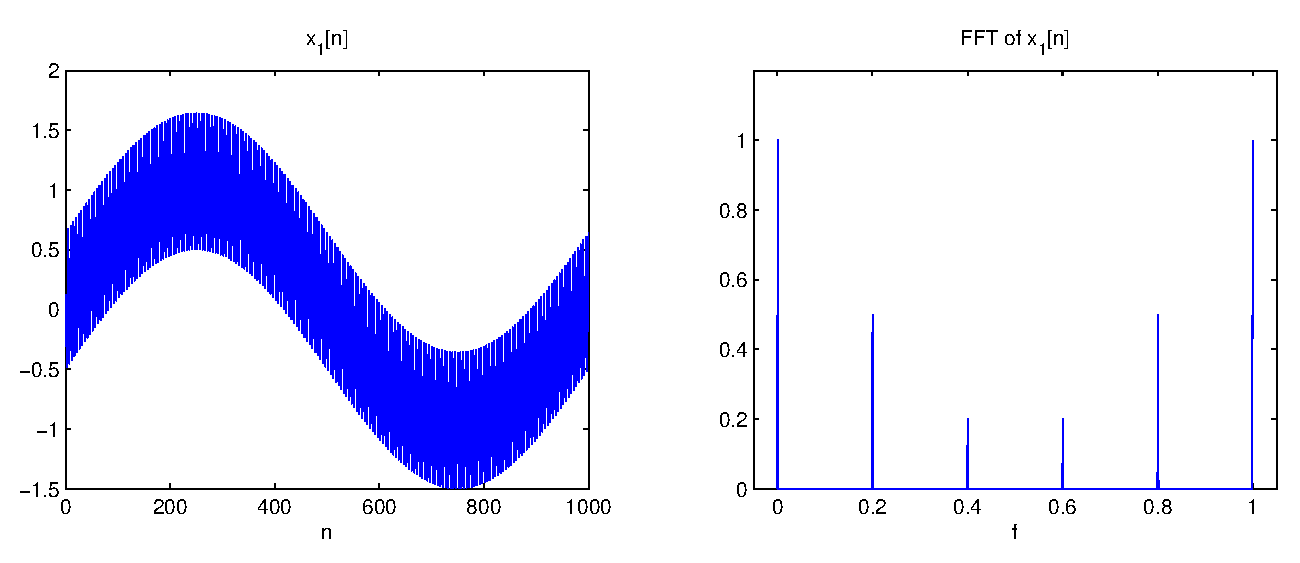
\includegraphics[scale=0.6]{./img/sins.eps}
    \caption{The function $x_1[n]$ (left) and its DFT (right). Notice that the DFT shows spikes at the frequency of each sinusoid in the signal, and also at the mirrored location $f'=f_{max}-f$, where $f_{max}=1/T_s$. Because of this mirroring, unique frequencies can only be represented up to $f_N=1/(2T_s)$, which is known as the Nyquist frequency.}
    \label{decomp1}
\end{figure}
\begin{figure}
    \centering
    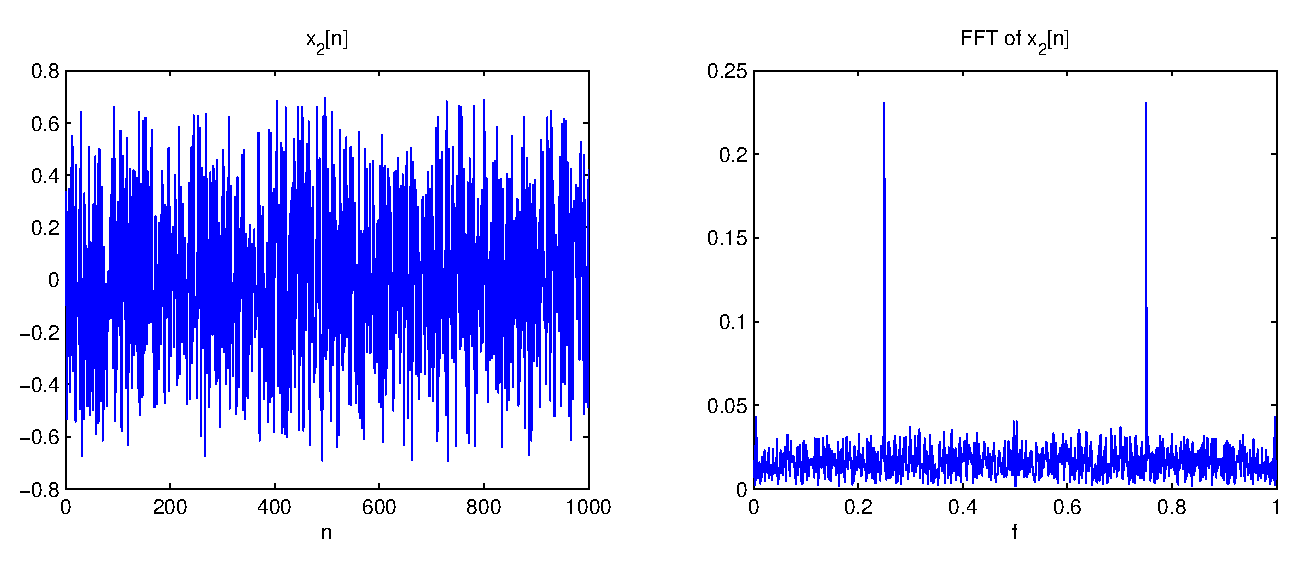
\includegraphics[scale=0.6]{./img/random.eps}
    \caption{The function $x_2[n]$ (left) and its DFT (right). Notice that the DFT show the spike at $f_0=0.25$Hz, and its mirror. This illustrates one of the advantages of the DFT: though it was difficult to spot the sinusoidal oscillation in the time-domain signal (left), it sticks out quite clearly in the frequency domain (right).}
    \label{decomp2}
\end{figure}


\subsection{Symmetry in the FFT Algorithm}
\label{fftSymmetry}
The symmetry seen in the Cooley-Tukey FFT algorithm (lines 11 and 12 in the code listing from section \ref{fftRecursive}) can be explained by exploiting symmetry of the DFT:
\begin{align*}
X[k+N/2] &= \sum_{n=0}^{N/2-1}x_e[n]e^{-i2\pi n (k+N/2) /(N/2)} + e^{-i2\pi (k+N/2)/N}\sum_{n=0}^{N/2}x_o[n]e^{-i2\pi n (k+N/2) /(N/2)}\\
&=\sum_{n=0}^{N/2-1}x_e[n]e^{-i2\pi n k/(N/2)}e^{-i2\pi n} + e^{-i2\pi k/N}e^{-i\pi}\sum_{n=0}^{N/2-1}x_o[n]e^{-i2\pi n k/(N/2)}e^{-i2\pi n}\\
&= \sum_{n=0}^{N/2-1}x_e[n]e^{-i2\pi n k/(N/2)} - e^{-i2\pi k/N}\sum_{n=0}^{N/2-1}x_o[n]e^{-i2\pi n k/(N/2)}\\
&= X_e[k] - e^{-i2\pi k/N}X_o[k]
\end{align*}